%%%%%%%%%%%%%%%%%%%%%%%%%%%%%%%%%%%%%%%%%%%%%%%%%%%%%%%%%%%%%%%%%%%%%%%%%%%%%%%
\section{INTRODUCTION}
%%%%%%%%%%%%%%%%%%%%%%%%%%%%%%%%%%%%%%%%%%%%%%%%%%%%%%%%%%%%%%%%%%%%%%%%%%%%%%%

%%%%%%%%%%%%%%%%%%%%%%%%%%%%%%%%%%%%%%%%%%%%%%%%%%%%%%%%%%%%%%%%%%%%%%%%%%%%%%%
\subsection{Solar-powered UAVs for perpetual flight endurance}
%%%%%%%%%%%%%%%%%%%%%%%%%%%%%%%%%%%%%%%%%%%%%%%%%%%%%%%%%%%%%%%%%%%%%%%%%%%%%%%

When carefully designed, solar-electrically powered fixed-wing Unmanned Aerial Vehicles (UAVs) exhibit significantly increased flight endurance over purely-electrically or even gas-powered aerial vehicles. Given certain environmental conditions, a solar-powered UAV creates surplus energy when observed over a full day-night cycle, i.e. it will fully recharge its batteries during the day to continue flight through the night and potentially subsequent day-night cycles. Long endurance - and especially this multi-day continuous flight capability termed ``perpetual endurance'' - is of significant interest for large-scale mapping, observation or telecommunications relay applications as they occur in Search-And-Rescue (SAR) missions, industrial or agricultural inspection, meteorological surveys, border patrol and more \cite{NASA_Pathfinder}.
 
Recently, interest in employing solar-powered large-scale (wing span above 20m) High-Altitude Long-Endurance (HALE) UAVs as ``atmospheric satellites'' - i.e. stationary/loitering platforms e.g. for telecommunications relay - has peaked. Notable examples of this trend are Solara \cite{IEEE_AtmosphericSatellites} and Zephyr, the latter of which has already demonstrated a continuous flight of 14 days\cite{QinetiQ_Zephyr14dayRecord}. In contrast, smaller scale solar-powered UAVs are mostly designed for Low-Altitude Long Endurance (LALE) applications. While they have to cope with the more challenging meteorological phenomenas of the lower atmosphere (clouds, rain, wind gusts or thermals), they generally have the advantage of lower complexity and cost as well as easier and faster handling (e.g. through hand-launchability) as beneficial in First-Aid SAR scenarios. However, research in small-scale solar UAVs targeting perpetual endurance has been relatively sparse, with most research including \cite{Morton_ICRA2013} focussing on conceptual design studies without extensive flight experience. However, in 2005, Cocconi's SoLong \cite{Cocconi_SoLong} performed a continuous 48 hours flight using solar power and thermal-updraft hunting, though with limited airplane autonomy. Noth\cite{Noth_PhD} presents the conceptual design methods, realization and experimental flight results of the 3.2m wing span ``SkySailor'', which demonstrated a 27 hours solar-powered continuous flight without the use of thermals in 2008. 
\begin{figure}[h]
    \centering
    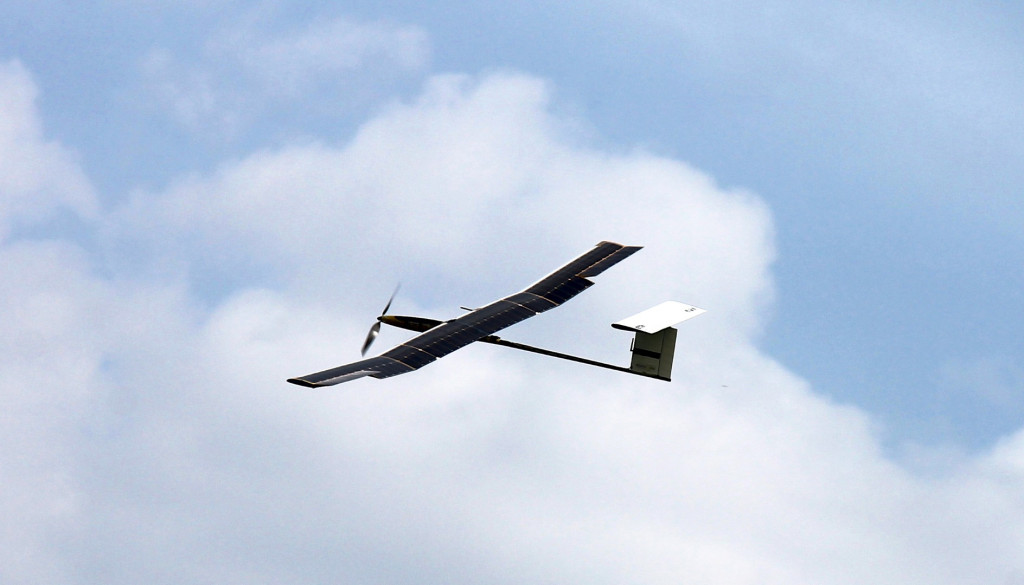
\includegraphics[width=\linewidth]{images/1_AtlantikSolarCollage}
    \caption{The AtlantikSolar solar-powered UAV developed at ETH Zurich}
    \label{fig:AtlantikSolarCollage}
\end{figure}

%%%%%%%%%%%%%%%%%%%%%%%%%%%%%%%%%%%%%%%%%%%%%%%%%%%%%%%%%%%%%%%%%%%%%%%%%%%%%%%
\subsection{Contributions of this paper}
%%%%%%%%%%%%%%%%%%%%%%%%%%%%%%%%%%%%%%%%%%%%%%%%%%%%%%%%%%%%%%%%%%%%%%%%%%%%%%%

This paper aims to extend the work of \cite{Cocconi_SoLong,Noth_PhD} by presenting AtlantikSolar, a solar-powered LALE-UAV with a wing span of 5.6m designed towards more robust multi-day autonomous operation capabilities while providing the option to use an advanced optical\&infrared sensor system together with on-board computation ressources developed at ETH Zurich. The contribution of the paper lies in presenting the complete development cycle from conceptual UAV design to actual testing and missions, or more specifically
  
 \begin{enumerate}
\item The application and extension of the conceptual design approach in \cite{Noth_PhD,Leutenegger_JIRS} towards more robust multi-day flight under sub-optimal meteorological conditions
\item The realization of the conceptual design in UAV hardware, i.e. structure, low-level electronics \& avionics 
\item The development of onboard EKF state estimation algorithms and flight control methods based on PID control with non-linear guidance
\item The discussion of flight test results including long-endurance flight (up to 12h) and mapping results during exemplary Search-And-Rescue missions.
\end{enumerate}

%+ picture of AtlantikSolar in flight
%1) Kostas from side
%2) ``Aerobatic picture'' from TJ
%3) Maybe landing picture.
%- Make sure to include some with sensor pod